\documentclass[12pt,a4paper]{article}

\usepackage{graphicx}% Include figure files
\usepackage{dcolumn}% Align table columns on decimal point
\usepackage{bm}% bold math
%\usepackage{hyperref}% add hypertext capabilities
%\usepackage[mathlines]{lineno}% Enable numbering of text and display math
%\linenumbers\relax % Commence numbering lines

%\usepackage[showframe,%Uncomment any one of the following lines to test 
%%scale=0.7, marginratio={1:1, 2:3}, ignoreall,% default settings
%%text={7in,10in},centering,
%%margin=1.5in,
%%total={6.5in,8.75in}, top=1.2in, left=0.9in, includefoot,
%%height=10in,a5paper,hmargin={3cm,0.8in},
%]{geometry}

\usepackage{multicol}%Para hacer varias columnas
\usepackage{multicol,caption}
\usepackage{multirow}
\usepackage{cancel}
\usepackage{hyperref}
\hypersetup{
    colorlinks=true,
    linkcolor=blue,
    filecolor=magenta,      
    urlcolor=cyan,
}

\setlength{\topmargin}{-1.0in}
\setlength{\oddsidemargin}{-0.3pc}
\setlength{\evensidemargin}{-0.3pc}
\setlength{\textwidth}{6.75in}
\setlength{\textheight}{9.5in}
\setlength{\parskip}{0.5pc}

\usepackage[utf8]{inputenc}
\usepackage{expl3,xparse,xcoffins,titling,kantlipsum}
\usepackage{graphicx}
\usepackage{xcolor} 
\usepackage{nopageno}
\usepackage{lettrine}
\usepackage{caption}
\renewcommand{\figurename}{Figura}
\usepackage{float}
\renewcommand\refname{Bibliograf\'ia}
\usepackage{amssymb}
\usepackage{amsmath}
\usepackage[rightcaption]{sidecap}
\usepackage[spanish]{babel}

\providecommand{\abs}[1]{\lvert#1\rvert}
\providecommand{\norm}[1]{\lVert#1\rVert}

% CABECERA Y PIE DE PÁGINA %%%%%
\usepackage{fancyhdr}
\pagestyle{fancy}
\fancyhf{}

\begin{document}

\begin{enumerate}
    \item Haz un programa en F90 que resuelva la ecuación de segundo grado, donde a, b y c son los coeficientes de la ecuación y se consideran como números reales solamente, toma en cuenta los casos cuando a=0, si es así el programa deberá poner el letrero en este caso “la ecuación es lineal y la raíz es :” y dar el resultado, si a=0 y b=0 poner el letrero “no hay solución”, considerarás también los casos cuando el discriminante es igual a cero, mayor que cero y menor que cero, si es cero el programa deberá escribir en pantalla “la raíz es doble” y deberá obtener la raíz, si es mayor a cero deberá obtener las dos raíces y si el discriminante es menor que cero, poner el letrero “no hay raíces reales” y obtener las soluciones complejas.
    
    \begin{verbatim}
PROGRAM Chicharronera
IMPLICIT NONE 
REAL :: a, b, c, det, x_1, x_2
COMPLEX :: x_1_cmplx, x_2_cmplx

! Este programa recibe como parametros 3 nùmeros reales de precisiòn
!sencilla que representan los coeficientes de una ecuaciòn cuadràtica,
! tambien se usan otras variables del mismo tipo y precisiòn como auxiliares
! para presentar las raìces de dicho polinomio

WRITE (*,*) "Ingresa el coeficiente cuadràtico"
READ (*,*) a
		
WRITE (*,*) "Ingrese el coeficiente lineal"
READ (*,*) b

WRITE (*,*) "Ingrese el tèrmino independiente"
READ (*,*) c

det = b**2 - 4*a*c !variable auxiliar

IF ((a /= 0) ) THEN !sirve para comprobar que sea una ecuaciòn de segundo grado

IF (det > 0) THEN!raices reales
			
x_1 = (-b + sqrt(det)) / (2*a) !raìz 1
x_2 = (-b - sqrt(det)) / (2*a) !raiz 2	

WRITE (*,*) "Las raìces del polinomio"
WRITE (*,*) a, "x**2 +", b, "x +", c
WRITE (*,*) "son:"
WRITE (*,*) "------------------------------------------------"
WRITE (*,*) x_1, x_2	

ELSE IF (det < 0) THEN!raices complejas

x_1_cmplx = cmplx(-b/(2*a), sqrt(-det) / (2*a)) !raìz 1
x_2_cmplx = cmplx(-b/(2*a),-sqrt(-det)/(2*a)) !raiz 2

WRITE (*,*) "Las raìces del polinomio"
WRITE (*,*) a, "x**2 +", b, "x +", c
WRITE (*,*) "son:"
WRITE (*,*) "------------------------------------------------"
WRITE (*,*) x_1_cmplx, x_2_cmplx
	
ELSE IF (det == 0) THEN!raiz doble

x_1 = -b / (2*a)	
	
WRITE (*,*) "La raíz es doble"
WRITE (*,*) "La raìz del polinomio"
WRITE (*,*) a, "x**2 +", b, "x +", c
WRITE (*,*) "es:"
WRITE (*,*) "------------------------------------------------"
WRITE (*,*) x_1
		
END IF

ELSE IF (a == 0 .AND. b /= 0) THEN!lineal

x_1 = -c/b

WRITE (*,*) "La ecuación es lineal y la raíz es:",  x_1

ELSE IF (a == 0 .AND. b == 0) THEN!sin solución
WRITE (*,*) "No hay solución"

END IF

END PROGRAM Chicharronera
    \end{verbatim}
    
    \begin{figure}
        \centering
        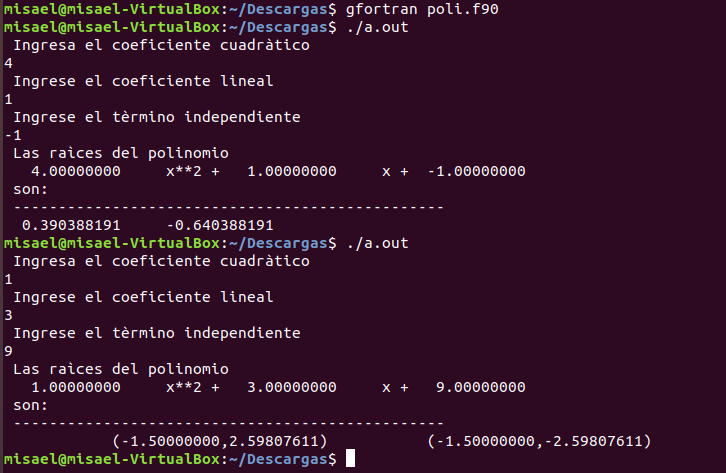
\includegraphics[scale = 0.5]{1.1.1.PNG}
    \end{figure}
    
    \begin{figure}
        \centering
        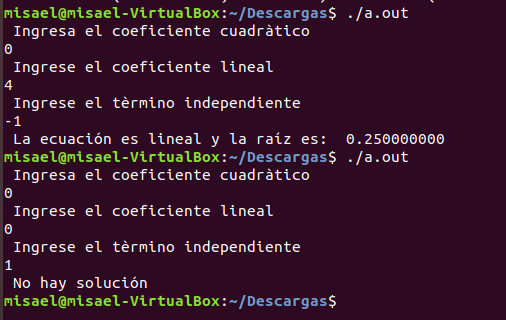
\includegraphics[scale = 0.5]{1.1.2.PNG}
    \end{figure}
    
    
    Los resultados obtenidos coinciden con los resultados arrojados por Wolfram, así que debe estar bien
    
    \begin{figure}
        \centering
        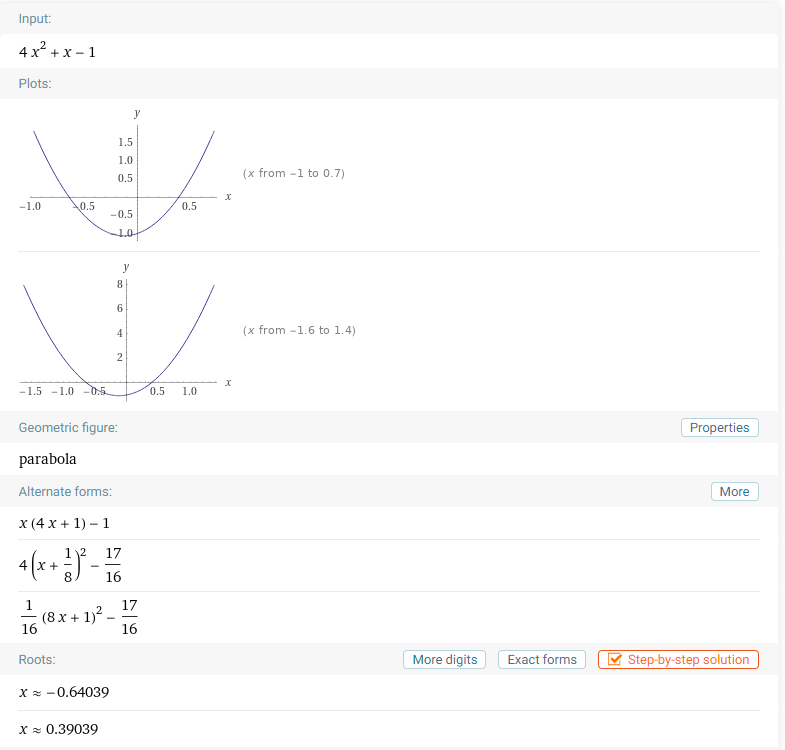
\includegraphics[scale = 0.5]{1.1.PNG}
    \end{figure}
    
    \newpage
    
    \begin{figure}
        \centering
        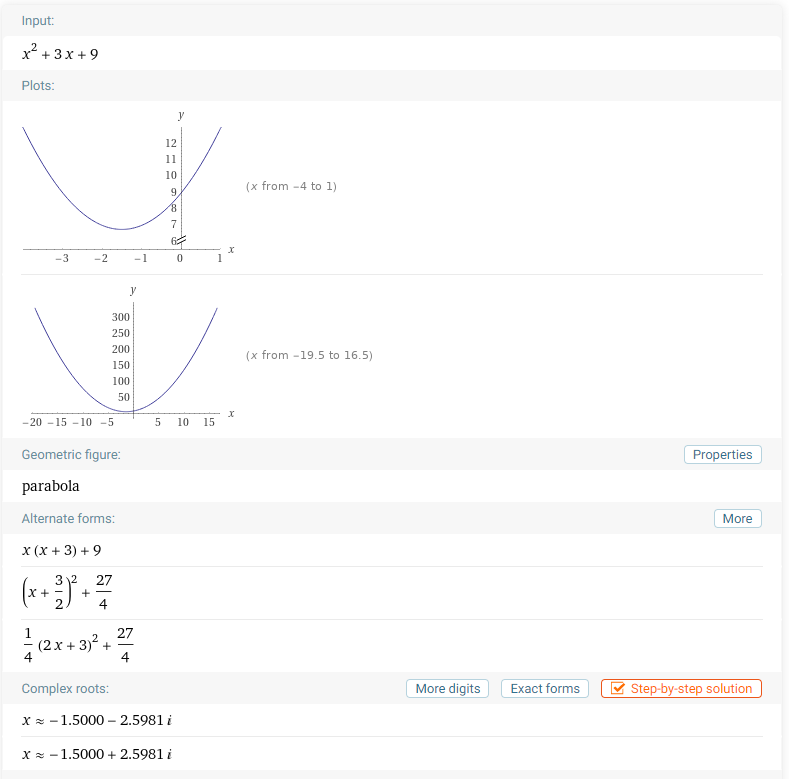
\includegraphics[scale = 0.5]{1.2.2.PNG}
    \end{figure}
    
    \begin{figure}[h]
        \centering
        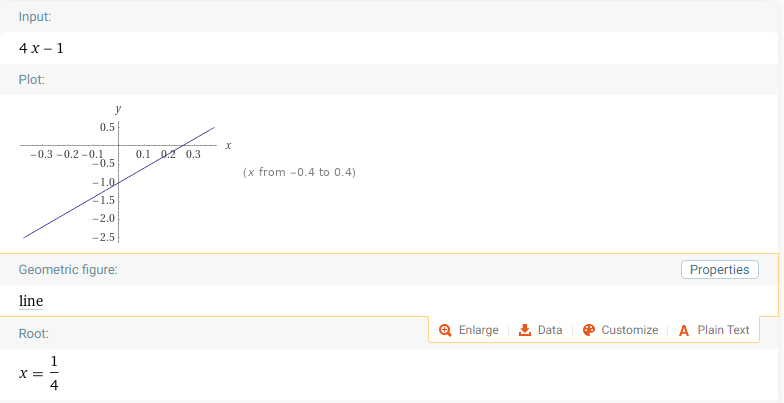
\includegraphics[scale = 0.5]{1.2.3.PNG}
    \end{figure}
    
    \newpage
    
    \item Haz un programa en F90 que resuelva la serie de Taylor del coseno, hasta un número dado de términos y un argumento x, los cuales son la entrada del programa,
    

    
    \begin{equation*}
    \cos{x} = \sum_{n=0}^{\infty}(-1)^{n} \frac{x^{2n}}{(2n)!}
    \end{equation*}
    
    considera que para cambiar el signo en los términos, en f90 puede usarse: (-1)**i donde i es un contador, deberás usar dos “do’s anidados” (uno para llevar la suma y otro para el factorial). Compara los resultados de tu programa con los obtenidos por la función intrínseca cos(x).
    
        \begin{verbatim}
program taylor
implicit none
real, parameter :: pi = 3.14159265359
integer, parameter :: extra = selected_real_kind(p=24,r=1000)
integer :: i, j, m, k, y, z
real(extra), dimension(2000) :: fact, coss
real(extra) :: x, xx, realcos, scos = 1
!serie de taylor alrededor del 0 (serie de Mclaurin) para aproximar el coseno
!en cualquier valor gracias a la traslación se que usa


write (*,*) "¿Cual es el valor que quieres evaluar?(en radianes)"
read (*,*) x

y = floor(x/pi)
z = modulo(y,2)

if (abs(x) .GT. 2*pi) then !traslación para evitar que algún dato de la serie explote
	xx = x - ((y-z)*pi)

else if (abs(x) .LE.2* pi) then
		xx = x
end if

fact(1) = 1

do i = 2, 2000, 1 !calculo de los factoriales necesarios
	fact(i) = fact(i-1) * (i)
end  do

do i = 1, 1000, 1 !elementos de la serie
	
	coss(i) = ((-1)**i) * ((xx**(2*i))/(fact(2*i)))
end do

do i = 1, 1000, 1 !suma de todos los elementos
	scos = scos + coss(i)
end do

realcos = cos(x) !coseno "real"
	
write (*,*)"El valor aproximado es : ", scos
write (*,*) "El valor 'real' es : ", realcos

end program taylor
    \end{verbatim}
    
    Los valores aproximados son muy parecidos a los obtenidos con la función intrínseca tanto para valores grandes y negativos
    
    \begin{figure}[h!]
        \centering
        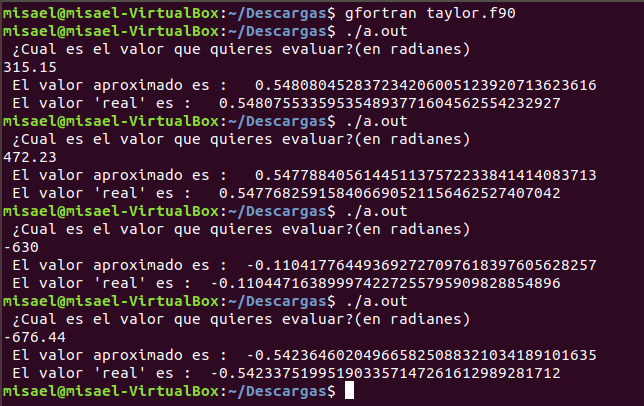
\includegraphics[scale = 0.7]{2.1.1.PNG}
    \end{figure}
    
     
    
    
    \item Haz un programa en F90 que dado un numero $n > 2$ obtenga todos los primos anteriores.
    
    \begin{verbatim}
program primos
implicit none
integer :: n, i, k, cuenta
!programa que muestra los numeros primos anteriores al ingresado

write (*,*) "ingresa un entero mayor a 2"
read (*,*) n

if (n .GT. 2) then 
	
	do i = n, 2, -1
		cuenta = 0
		do k = i, 2, -1
			if (modulo(i,k) .EQ. 0) then
				cuenta = cuenta+1
			end if
		end do
		if (cuenta .EQ. 1) then
			write (*,*) i
		end if
	end do
	
else 

	write (*,*) "no es un numero mayor a 2"

end if


end program primos
    \end{verbatim}
    
    Los primeros 100 números primos que nos da el programa son los mismo que dice Wolfram, por lo que debe estar bien
    
    \begin{figure}[h!]
        \centering
        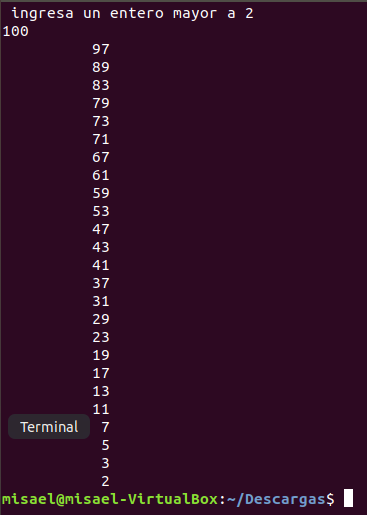
\includegraphics[scale = 0.7]{3.1.PNG}
    \end{figure}
    
    \begin{figure}[h!]
        \centering
        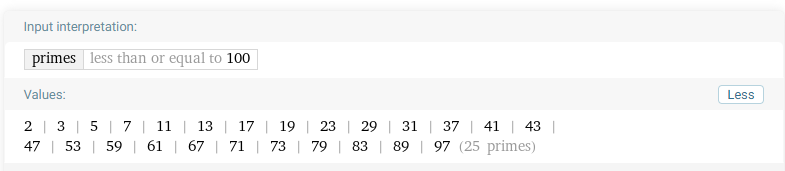
\includegraphics[scale = 0.7]{3.2.PNG}
    \end{figure}
    
    \item Haz un programa en F90 que realice mínimos cuadrados lineales con los datos obtenidos de un archivo con $<$ puedes usar el imports-85.data cortando las columnas 13 y 26. Compara tus resultados con los obtenidos en gnuplot.
    
    \begin{verbatim}
program min

character(10) :: a(205,26)
integer :: i,j
real :: x(205), y(205)

do i = 1, 205
	read (*,*) (a(i,j), j= 1, 26)
end do


do i = 1, 205
	read(a(i,13), *) x(i)
	read(a(i,26), *) y(i)
end do

print*, "b = ", (sum(y)*sum(x*x)-sum(x)*sum(x*y))/(205*sum(x*x)-sum(x)*sum(x))
print*, "m = ", (205*sum(x*y)-sum(x)*sum(y))/(205*sum(x*x)-sum(x)*sum(x))

end program min
    \end{verbatim}
    
    El programa es el mismo que el de clase y la gráfica parece ajustarse bien a los datos, así que igual debe estar bien
    
    \begin{figure}[h!]
        \centering
        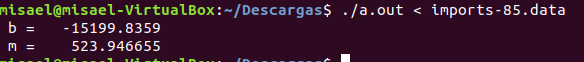
\includegraphics[scale = 0.7]{4.1.PNG}
    \end{figure}
    
    \begin{figure}[h!]
        \centering
        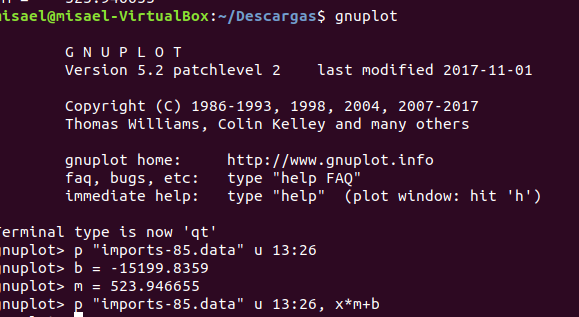
\includegraphics[scale = 0.7]{4.2.PNG}
    \end{figure}
    
    \begin{figure}[h!]
        \centering
        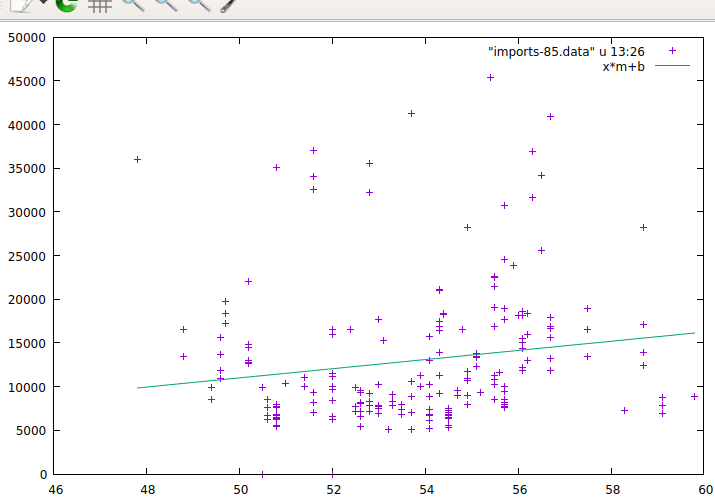
\includegraphics[scale = 0.7]{4.3.PNG}
    \end{figure}

\end{enumerate}

\end{document}
